\chapter{Introduction}
\label{chap:introduction}
%%%%%%%%%%%%%%%%%%%%%%%%%%%%%%%%%%%%%%%%%%%%%%%%%%%%%%%%%%%%%%%%

%%%%%%%%%%%%%%%%%%%%%%%%%%%%%%%%%%%%%%%%%%%%%%%%%%%%%%%%%%%%%%%%
\section{Motivation}
%%%%%%%%%%%%%%%%%%%%%%%%%%%%%%%%%%%%%%%%%%%%%%%%%%%%%%%%%%%%%%%%
Bla bla bla...

Include references: \cite{cover} and \cite{telatar,tse,costa}.

I want to reference this \cite{RaphaelPaper}. 


\subsection{Mathematics}
%=================================
An important formula is
\[ f(z) = a(x,y) + \cmplx \cdot b(x,y).
\]

A numbered formula that can be referenced \eqref{eq:formula1} is 
\begin{equation}
\label{eq:formula1}
\frac{d f}{d z} = \lim_{z \to z_0}\frac{f(z)-f(z_0)}{z - z_0} = \lim_{\Delta z \to 0}\frac{f(z_0 + \Delta z)- f(z_0)}{\Delta z}.
\end{equation}



\subsection{Tables and Figures}
%=================================

Table \ref{tbl:Values1} shows interesting numbers.

%-------------------------------------------------------------
\begin{table}[h]
\begin{center}
\label{blaq1}
  \begin{tabular}{| l || c | r |} \hline
  Value type & Node 1 & Node 2 \\ \hline \hline
  Value 1 & 1 & 2 				\\ \hline
  Value 2 & 3 & 4 				\\ \hline
\end{tabular}
\caption{Values for nodes.}
\label{tbl:Values1}
\end{center}
\end{table}
%-------------------------------------------------------------

Algorithm \ref{algo:algorithm1} summarizes a iterative gradient search.

%-------------------------------------------------------------
\begin{algorithm}[h!]
\caption[Algorithm 1]{\!\!\textbf{:} Steepest Ascent}
\label{algo:algorithm1}
\begin{algorithmic}[1]
\STATE \texttt{Given:} a starting point $\bmz[0]$, randomly chosen
\STATE \texttt{Repeat:}
\STATE \qquad $m \leftarrow m+1$
\STATE \qquad \texttt{Search direction:} $\bDelta[m] = \nabla_{\bmz^*} f\left( \bmz[m] \right)$
\STATE \qquad \texttt{Update:} $\bmz[m+1] = \bmz[m] + \mu \cdot \bDelta[m]$
\STATE \texttt{Until:} stopping criterion is satisfied
\STATE \texttt{Return:} $\bmz[m+1] \approx \bmz_\text{opt}$
\end{algorithmic}
\end{algorithm}
%-------------------------------------------------------------

Some results are plotted in Fig. \ref{fig:Plot1}. 

%-------------------------------------------------------------
\begin{figure}[h]
\begin{center}
  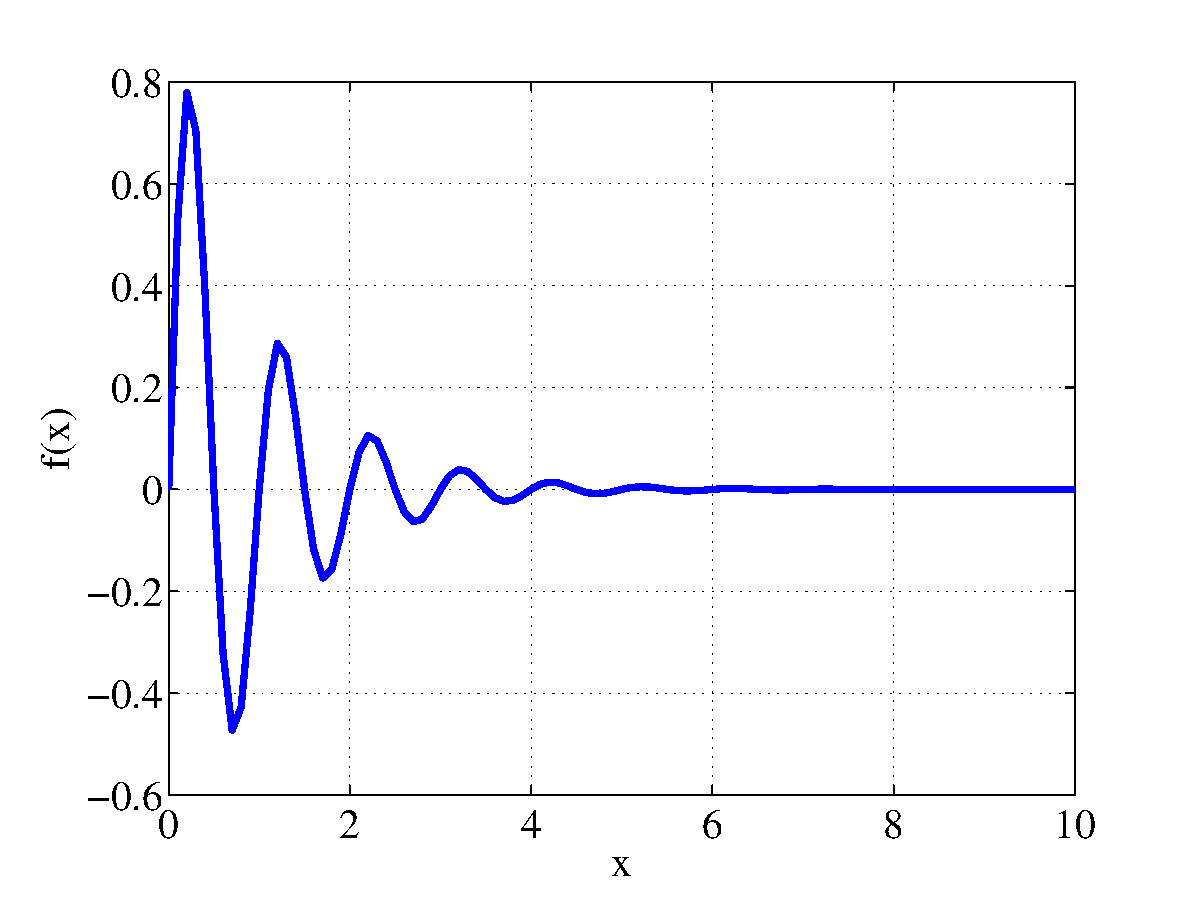
\epsfig{file=figures/Plot1, width=0.7\textwidth}
\end{center}
\caption{A signal.}
\label{fig:Plot1}
\end{figure}
%-------------------------------------------------------------

%%%%%%%%%%%%%%%%%%%%%%%%%%%%%%%%%%%%%%%%%%%%%%%%%%%%%%%%%%%%
%%% E N D   of   C H A P T E R 
%%%%%%%%%%%%%%%%%%%%%%%%%%%%%%%%%%%%%%%%%%%%%%%%%%%%%%%%%%%%